\documentclass[xcolor=table, aspectratio=169, bigger, handout]{beamer}

\usepackage{shyne}

% Theme settings
\setbeamertemplate{navigation symbols}{}

\usetheme{Madrid}
\usefonttheme{structurebold}
\usefonttheme[onlymath]{serif}

\AtBeginSection[]
{ 	\begin{frame}{}

	{
	\usebeamerfont{frametitle}
	\begin{beamercolorbox}
		[wd={\textwidth}, center, sep=.2in, rounded=true, shadow=true]
		{frametitle}
	Week \thesection\\  \secname 
	\end{beamercolorbox}
	}
	
	\end{frame} 
}

\AtBeginSubsection[]
{ 	\begin{frame}{}

	{
	\usebeamerfont{frametitle}
	\begin{beamercolorbox}
		[wd={\textwidth}, center, sep=.2in, rounded=true, shadow=true]
		{frametitle}
	Section \thesection .\thesubsection\\  \subsecname 
	\end{beamercolorbox}
	}
	
	\end{frame} 
}

\title[Week 8]{Stat 201: Statistics I\\Week 8 }
\author[M. Shyne]{}
\institute[Metro State]{
\includegraphics[width=1.75in]{../images/metro_logo}}
\date[3/24/2019]{
\\ \bigskip \bigskip 
\includegraphics[width=.4in]{../images/cc_big}}



\begin{document}
\frame{\titlepage}

% Week 8
\setcounter{section}{7}
\section{Hypothesis Testing}

%
% Section 8.1
%
\subsection{More on Confidence Intervals}


%%%%%%%%%%

\begin{frame}{Sample size}
\begin{block}{}
A confidence interval defines a region of probable values for a population parameter. Often, it is desirable to design an experiment which will estimate a population parameter within a specified accuracy. The sample size needed to achieve a desired margin of error can be calculated.
\end{block}
\end{frame}


%%%%%%%%%%
\begin{frame}{Calculating sample size}
\begin{block}{}
Recall, a confidence interval is defined as,\\ \smallskip
\eq{CI(1-\alpha)\% = x \pm ME} \smallskip
where the margin of error is calculated by,\\ \smallskip
\eq{ME = z_{\alpha/2} \Paren{\frac s {\sqrt n}}} \smallskip
Solving for $n$ (sample size) results in, after some algebra,\\ \smallskip
\eq{ n = \Paren{\frac {s \times z_{\alpha/2}}{ME}}^2}
\end{block}
\end{frame}


%%%%%%%%%%
\begin{frame}{Calculating sample size, cont.}
\begin{block}{}
\eq{ n = \Paren{\frac {s \times z_{\alpha/2}}{ME}}^2} \medskip

A sample size calculation requires the following values:
\begin{itemize}
\pause \item The critical value $z_{\alpha/2}$ specified by the desired confidence level $(1-\alpha)\%$

\pause \item The desired accuracy of the estimate specified by an acceptable margin of error

\pause \item The sample standard deviation $s$. Finding a suitable value for $s$ is often the most difficult part of a sample size calculation.

\end{itemize}

\end{block}
\end{frame}

%%%%%%%%%%
\begin{frame}{Standard deviations for means}
\begin{block}{}
A reasonable estimate for sample standard deviation must be determined when calculation sample sizes for confidence intervals of means.\\ \medskip

Possible sources:
\begin{itemize}
\pause \item Known population values

\pause\item Previous published studies

\pause\item Pilot studies

\pause \item Sometimes a sample size calculation is performed using a margin of error defined as a proportion of an unknown stand deviation (i.e. a margin of error of half a standard deviation)
\end{itemize}

\end{block}
\end{frame}

%%%%%%%%%%
\begin{frame}{Standard deviations for proportions}
\begin{block}{}
When working with proportions and binomial distributions, standard deviations are calculated from the sample probability or proportion rather than measured directly from the data. Thus, a reasonable estimate of the sample proportion is required.\\ \medskip

\begin{itemize}
\pause \item Proportion estimates may be estimated from previous work or known values in a similar manner as standard deviations for means

\pause\item If no reasonable estimate can be made, a conservative value of $\hat p = 0.5$ should be used.
\end{itemize}

Then, the sample size calculation for a confidence interval of proportions in,\\ \smallskip

\eq{n = \Paren{\frac{\sqrt{\hat p \times (1-\hat p)} \times z_{\alpha/2}}{ME}}^2 = \hat p \times (1-\hat p) \times \Paren{\frac{ z_{\alpha/2}}{ME}}^2}
\end{block}
\end{frame}

%%%%%%%%%%
\begin{frame}{Calculating sample size, example}
\begin{exampleblock}{Example}
Metro State wants to know the mean height of its male students within $\pm 2$ inches with 95\% confidence. How large of a sample is required to get the desired results? \\ \smallskip

\begin{itemize}
\pause\item A 95\% confidence level means $\alpha = 0.05$ and $z_{\alpha/2} = 1.96$

\pause\item The desired margin of error is 2 inches

\pause\item Previous studies have estimated the mean height of adult males in the U.S. is 69.2 inches with a standard deviation of 5.79.
\end{itemize}

\pause Then, \\ \smallskip
\eq{n = \Paren{\frac {s \times z_{\alpha/2}}{ME}}^2 = \Paren{\frac {5.79 \times 1.96}{2}}^2 = 32.197 \implies 33} \smallskip

\begin{itemize}
\pause\item Calculated sample sizes should always be rounded \bt{up}.
\end{itemize}
\end{exampleblock}
\end{frame}

%%%%%%%%%%
\begin{frame}{Confidence intervals as inference}
\begin{block}{}
A confidence interval from a sample can be used to determine whether population the sample was drawn from has a parameter that  matches a value of interest.
\begin{itemize}
\pause\item If the value of interest \bt{is not} contained within the confidence interval, then there is evidence that the population parameter differs from the value.

\pause\item If the value if interest \bt{is} contained within the confidence interval, then there is not evidence the the parameter differs from the value. [Note: this is not the same as saying there is evidence that the parameter is the same as the value.]
\end{itemize} 
\end{block}
\end{frame}

%%%%%%%%%%
\begin{frame}{Confidence intervals as inference, example}
\begin{exampleblock}{Example}
Suppose Metro State conducts a study of height of male students which results in a 95\% confidence interval of (63.3, 67.9). What can be said about Metro State students as compared to the general U.S. population?
\begin{itemize}
\pause\item Since the mean height of U.S. males, 69.2 inches, is not contained in the confidence interval, there is evidence that Metro State students differ from the general U.S. population. 
\end{itemize}
\end{exampleblock}
\end{frame}

%%%%%%%%%%
\begin{frame}<handout:0>{Group work}
\begin{block}{}
\large
\begin{itemize}
\item For all questions, complete parts (a) and (b).
\end{itemize}
\end{block}
\end{frame}

%
% Section 8.2
%
\subsection{Basics of Hypothesis Testing}

%%%%%%%%%%
\begin{frame}{Statistical inference}
\begin{block}{}
Previously, statistics from random samples were used to learn something about populations by estimating population parameters. Knowledge about populations was inferred from the data of the sample.\\
\medskip
A similar question can be posed: Is a sample drawn from a population that is the same in an important way to a known population, or is the sample drawn from a population that is significantly different?
\end{block}

\end{frame}


%%%%%%%%%%
\begin{frame}{Hypothesis tests}
\begin{block}{}
An \bt{hypothesis test} is a formal statistical procedure to test claims about population parameters based on samples drawn from populations. Such claims, or \bt{hypotheses}, are often written as simple mathematical statements.\\
\medskip
It is important to be clear as to which population the claims or the tests are about,
\end{block}
\end{frame}

%%%%%%%%%%
\begin{frame}{Hypotheses, example}
\begin{exampleblock}{Example}
\begin{itemize}
\item Male Metro State students are shorter on average than the national mean of 69.2 inches.
\begin{itemize}
\pause\item Population: Male Metro State students
\pause\item $\mu < 69.2$
\end{itemize}

\pause\item The proportion of teen drivers who text or email while driving is 40\%
\begin{itemize}
\pause\item Population: Teen drivers
\pause\item $p = 0.4$
\end{itemize}

\pause\item A patient diagnosed with a particular rare disease has an expected survival time of 36 months. A new experimental treatment will extend the survival time.
\begin{itemize}
\pause\item Population: Patients with disease on experimental treatment
\pause\item $\mu > 36$
\end{itemize}
\end{itemize}
\end{exampleblock}
\end{frame}

%%%%%%%%%%
\begin{frame}{Hypotheses}
\begin{block}{}
The first step to conduct an hypothesis test is to identify two hypotheses.
\end{block}
\pause
\begin{block}{}
The \bt{null hypothesis} is the claim that nothing interesting has occurred, that a sub-population is \bt{not} different than the general population or that population parameters did \bt{not} change after treatment.
\end{block}
\pause
\begin{block}{} 
Conversely, the \bt{alternative hypothesis} is the claim that something interesting has occurred, that a sub-population is different or that parameters did change after treatment.
\end{block}
\pause
\begin{block}{}
Remember, both the null and alternative hypotheses are statements about populations, which will be tested using a sample.
\end{block}
\end{frame}

%%%%%%%%%%
\begin{frame}{Hypotheses, cont.}
\begin{block}{}
Null hypothesis:
\begin{itemize}
\item Denoted by $\bv{H_0}$
\item Always a statement that a parameter is \bt{equal to} some value
\item That value, denoted $p_0$ or $\mu_0$, is called the proportion or mean under the null hypothesis
\end{itemize}
\end{block}
\pause
\begin{block}{}
Alternative hypothesis:
\begin{itemize}
\item Denoted by $\bv{H_1}$ or $\bv{H_a}$ 
\item Can be a statement that a parameter is \bt{less than}, \bt{greater than} or \bt{not equal to} some value
\item Is usually a statement representing the research question
\end{itemize}
\end{block}
\end{frame}

%%%%%%%%%%
\begin{frame}{One-sided vs. two sided tests}
\begin{block}{}
If an alternative hypothesis has the form of a parameter being less than or greater than some value, the hypothesis test is called a \bt{one-sided test}.\\
\medskip
If an alternative hypothesis has the form of a parameter being not equal to some value, the hypothesis test is called a \bt{two-sided test}.
\end{block}
\end{frame}

%%%%%%%%%%
\begin{frame}{Hypotheses, example}
\begin{exampleblock}{Example}
Identify the null and alternative hypotheses, and whether it is a one-sided or two-sided test.\\
\pause\medskip
In the United States, adult men have a mean height of 69.2 inches. The Metro State administration want to do a study to see if male Metro State students are shorter than the general US population.

\begin{itemize}
\pause\item $H_0: \mu = 69.2 \qquad H_a: \mu < 69.2$\qquad One-sided

\end{itemize}

\pause\medskip
A patient diagnosed with a particular rare disease has an expected survival time of 36 months. A clinical trial is conducted to see if a new experimental treatment will change the survival time.
\begin{itemize}
\pause\item $H_0: \mu = 36 \qquad H_a: \mu \ne 36$\qquad Two-sided
\end{itemize}

\end{exampleblock}
\end{frame}

%%%%%%%%%%
\begin{frame}{Structure of hypothesis tests}
\begin{block}{}
Starting with null and alternative hypotheses derived from the research question and a random sample, all hypothesis tests have the same basic structure.
\begin{itemize}
\pause\item A test statistic is calculated which indicates the location of the sample within the sampling distribution, assuming the null hypothesis is true.

\pause\item The probability of getting a test statistic equal to or more extreme than the statistics belonging to the sample is calculated.

\pause\item If the calculated probability is below a pre-specified threshold, the null hypothesis is \bt{rejected} and it is said that there is evidence to support the alternative hypothesis.

\pause\item If the calculated probability is not below the pre-specified threshold, the null hypothesis is \bt{not rejected} and it is said that there is not evidence to support the alternative hypothesis.
\end{itemize}
\end{block}
\end{frame}

%%%%%%%%%%
\begin{frame}{P-values}
\begin{block}{}
In a hypothesis test, the \bt{p-value} is the probability of getting a sample with the test statistic or one more extreme, assuming the null hypothesis is true.
\begin{itemize}
\item Not to be confused with the population proportion $p$ or the probability function $P(A)$, though a p-value does represent a probability.
\end{itemize} 
\end{block}
\bigskip
{\centering
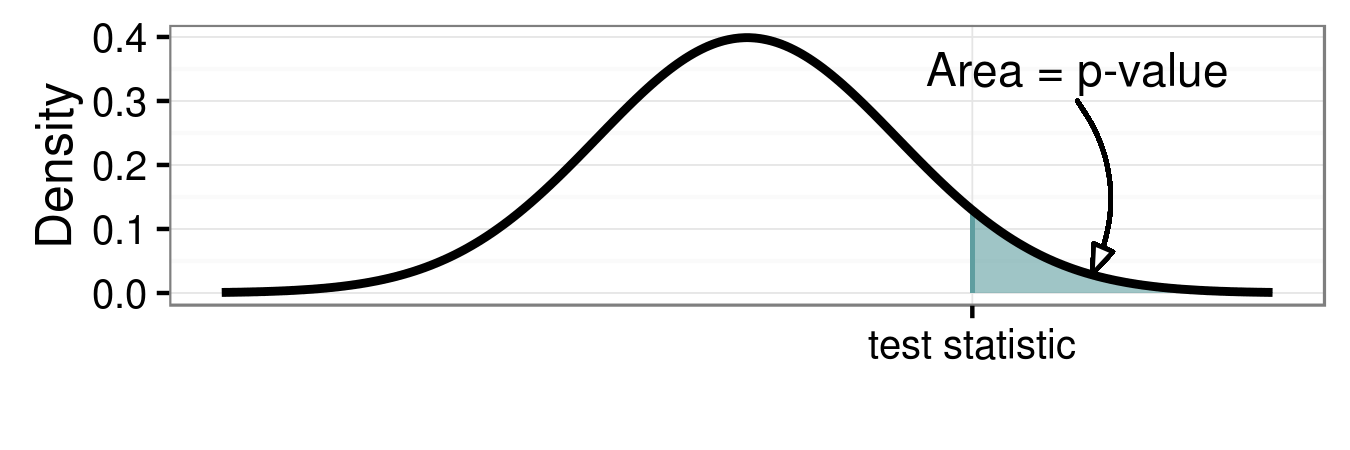
\includegraphics[width=4.5in]{../images/wk08_pvalue}
\par}

\end{frame}

%%%%%%%%%%
\begin{frame}{Calculating p-values}
\begin{block}{}
Calculating a p-value is that same as calculating probabilities in sampling distributions already learned.
\begin{itemize}
\pause\item Identify sampling distribution: 
\begin{itemize}
\item $z$ distribution for proportions
\item $t$ distribution for means
\end{itemize}
\pause\item Calculate \bt{test statistic}: $z$-score or $t$-score
\pause\item Find probability of test statistic or more extreme values in sampling distribution
\pause\item That probability is the p-value
\end{itemize}
\end{block}

\begin{block}{}
Luckily, all these steps can be accomplished easily with technology.
\end{block}
\end{frame}

%%%%%%%%%%
\begin{frame}{Significance level}
\begin{block}{}
Once the p-value is calculated, it is compared against a pre-specified threshold. This threshold is called the \bt{significance level} of the test.
\begin{itemize}
\pause\item Denoted by $\bv \alpha$
\pause\item This is the same $\alpha$ used for critical values and confidence intervals
\pause\item Thus, significance level can be thought of as an area in a sampling distribution
\pause\item Sometimes referred to as the rejection region
\end{itemize}
\end{block}
\end{frame}

%%%%%%%%%%
\begin{frame}{Significance level for one-sided test}
\begin{block}{}
In a one-sided test, the entire rejection region is located at one end of the distribution or the other.
\end{block}

\bigskip

{\centering
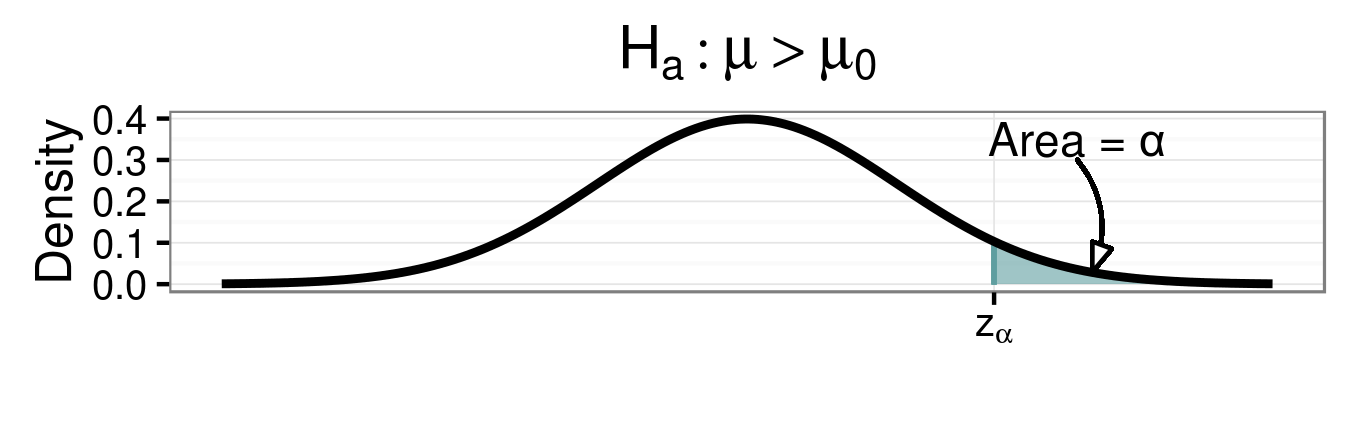
\includegraphics[width=5in]{../images/wk08_sig_up}
\par}
\end{frame}

%%%%%%%%%%
\begin{frame}{Significance level for two-sided test}
\begin{block}{}
In a two-sided test, the rejection region is split between the lower and upper extremes of the distribution.
\end{block}
\bigskip
{\centering
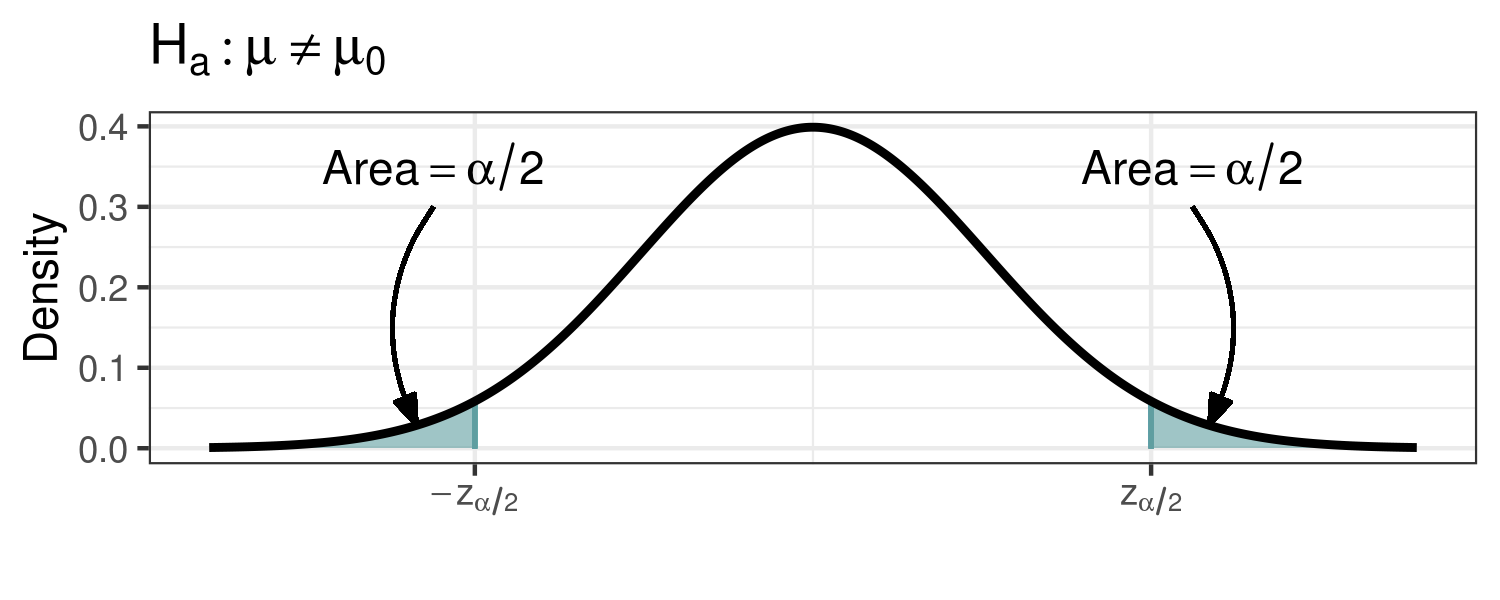
\includegraphics[width=5in]{../images/wk08_sig_2}
\par}

\end{frame}


%%%%%%%%%%
\begin{frame}{Stating conclusions}
\begin{block}{}
When reporting the results of an hypothesis tests, the following elements should be included:
\begin{itemize}
\pause\item Report the test statistic and p-value
\pause\item Report a decision on the null hypothesis based on the p-value and significance level ($\alpha$). 
\begin{itemize}
\item State the decision as ``Reject $H_0$" or ``Do not reject $H_0$".
\item The null hypothesis is never ``accepted".
\end{itemize}
\pause\item State the conclusion in terms of the research question
\begin{itemize}
\item ``There is evidence for..."
\item ``There is not evidence for..."
\end{itemize}
\end{itemize}
\end{block}
\end{frame}

%%%%%%%%%%
\begin{frame}{Stating conclusions, example}
\begin{exampleblock}{Example}
A study is conducted to test the claim that male Metro State students are shorter than the general population height of 69.2 inches. The test at a $\alpha=0.05$ level of significance produces a test statistic $t=-1.859$ and a p-value of $0.0358$. State the conclusion of the test.
\begin{itemize}
\pause\item $H_0: \mu=69.2, \qquad H_a: \mu < 69.2$
\pause\item $p=0.0358 < \alpha = 0.05$. Reject the null hypothesis. There is evidence to conclude that male Metro students are shorter than the general population.
\end{itemize}
\end{exampleblock}
\end{frame}

%%%%%%%%%%
\begin{frame}{Stating conclusions, example}
\begin{exampleblock}{Example}
A patient diagnosed with a particular rare disease has an expected survival time of 36 months. A clinical trial is conducted to see if a new experimental treatment will change the survival time. The hypothesis test at $\alpha = 0.01$ level of significance produces a p-value of 0.098. State the conclusion of the test.
\begin{itemize}
\pause\item $H_0: \mu = 36 \qquad H_a: \mu \ne 36$
\pause\item $p=0.098 > \alpha = 0.01$. Do not reject the null hypothesis. There is not evidence to conclude that the experimental treatment changes survival time.
\end{itemize}\end{exampleblock}
\end{frame}

%%%%%%%%%%
\begin{frame}{Steps for hypothesis test}
\begin{block}{}
\begin{enumerate}
\item Identify null and alternative hypotheses from research question
\item Determine appropriate sampling distribution
\item Calculate test statistic
\item Calculate p-value
\item Compare p-value to significance level $\alpha$ and report decision
\item State conclusion in terms of original research question
\end{enumerate}
Note: Steps 3 and 4 are often accomplished with technology
\end{block}
\end{frame}

%%%%%%%%%%
\begin{frame}{Making a decision with p-value}
\begin{block}{}
A \bt{small} p-value ($p < \alpha$) means a low probability of getting the observed sample if the null hypothesis is true. Thus, the null hypothesis is rejected.\\
\medskip
A \bt{large} p-value ($p > \alpha$) then means that the sample is not unlikely under the null hypothesis. Thus, the null hypothesis is not rejected.
\end{block}

\pause
\begin{alertblock}{To remember\ldots}
\large If p is low, the null must go.
\end{alertblock}

\end{frame}

%%%%%%%%%%
\begin{frame}{Or if this helps\ldots}

{\centering
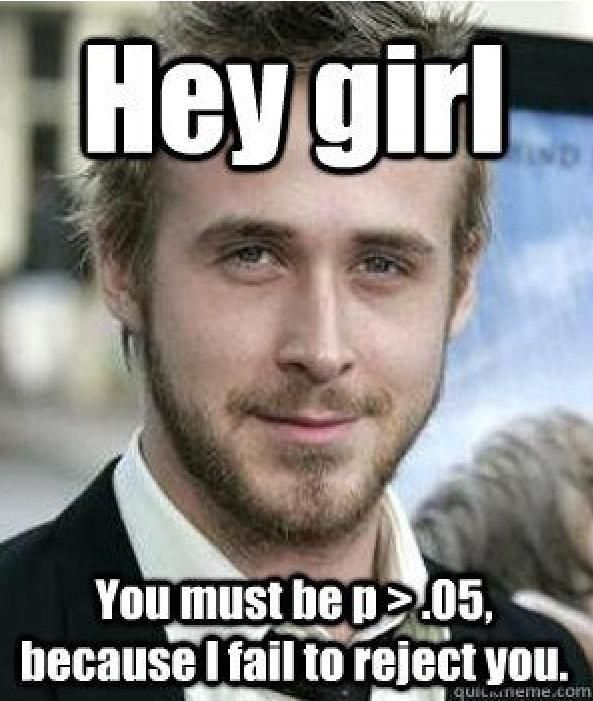
\includegraphics[width=2.35in]{../images/ch08_p_value_meme}
\par}

\end{frame}

%%%%%%%%%%
\begin{frame}{Critical value method}
\begin{block}{}
The hypothesis test procedure discussed thus far is known as the p-value method. An alternative method, known as the \bt{critical value} method, does not use p-values, but rather compares test statistics directly to appropriate critical values. If the test statistic is more extreme than the critical value, the null hypothesis is rejected.
\end{block}
\end{frame}

%%%%%%%%%%
\begin{frame}{Critical value method, example}
\begin{exampleblock}{Example}
A two-sided test with $\alpha = 0.05$ level of significance is conducted and results in a test statistic $z= - 2.8$.
\begin{itemize}
\item Recall, critical value $z_{\alpha/2} = \pm 1.96$.
\item Since $-2.8$ is more extreme than $-1.96$ ($-2.8 < -1.96$), reject the null hypothesis.
\end{itemize} 
\end{exampleblock}

\medskip
{\centering
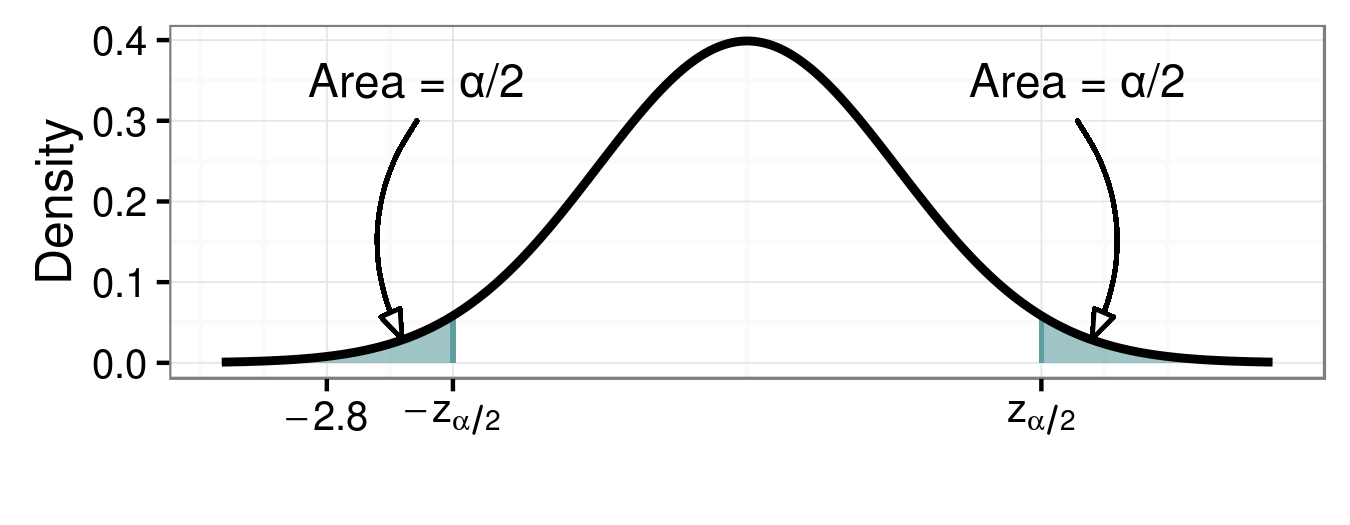
\includegraphics[width=4.5in]{../images/ch08_cv}
\par}

\end{frame}

%%%%%%%%%%
\begin{frame}{Types of errors in hypothesis tests}
\begin{block}{}
In an hypothesis test, either the null hypothesis is true or it is not, and either the null hypothesis is rejected or it is not. Thus, there are four possible outcomes.\\
\medskip
{\centering
\tabspacemed
\begin{tabular}{ r | c | c}
& Reject $H_0$ & Do not reject $H_0$\\
\hline
$H_0$ is true & Type I error ($\alpha$) & Correct decision\\
\hline
$H_0$ is not true & Correct decision & Type II error ($\beta$)
\end{tabular}
\tabspacedef
\par}
\medskip
\begin{itemize}
\pause\item A type I error occurs when the null hypothesis is rejected when it is in fact true. The probability of making a type I error in a test is designated $\alpha$.
\pause\item A type II error occurs when the null hypothesis is not rejected when it is in fact not true. The probability of making a type I error in a test is designated $\beta$.
\end{itemize}
\end{block}
\end{frame}

%%%%%%%%%%
\begin{frame}{Types of errors in hypothesis tests, cont.}
\begin{block}{}
\begin{itemize}
\item The acceptable probability of committing a type I error ($\alpha$), or level of significance,  is chosen prior to conducting a hypothesis test.
\pause\item The probability of committing a type II error ($\beta$) is determined by a number of factors, including the chosen $\alpha$ and the sample size.
\pause\item The probability of \bt{not} committing a type II error ($1-\beta$) is known as the \bt{power} of a test.
\pause\item There is a trade-off between $\alpha$ and $\beta$. Smaller $\alpha$ result in larger $\beta$ (and lower power) and vice versa.
\end{itemize}
\end{block}
\end{frame}

%%%%%%%%%%
\begin{frame}{Analogy to legal system}
\begin{block}{}
It can be useful to use a legal system analogy to help understand how hypothesis tests work. Consider a criminal trial:
\begin{itemize}
\pause\item A criminal defendant enters a trial with the \bt{presumption of innocence}. A defendant is assumed innocent until proven guilty.
\pause\item A prosecutor presents \bt{evidence} to show that the defendant should be considered guilty.
\pause\item The jury considers whether the evidence, when judged against a standard (\bt{beyond a reasonable doubt}), is sufficient to abandon the presumption of innocence.
\pause\item The jury returns a \bt{verdict}: either guilty or not guilty. A defendant is generally not declared innocent.   
\pause\item A jury can make two kinds of mistakes: they can convict an innocent defendant or they can fail to convict a guilty defendant.
\end{itemize}
\end{block}
\end{frame}

%%%%%%%%%%
\begin{frame}{Analogy to legal system, cont.}
\begin{block}{}
\begin{itemize}
\item The presumption of innocence is comparable to the \bt{null hypothesis}. An hypothesis tests begins by assuming that there is nothing interesting about the population(s) being studied.
\pause\item The evidence is comparable to the \bt{sample} collected to answer the research the question.
\pause\item The ``beyond a reasonable doubt" standard is comparable to the \bt{significance level} or $\bv \alpha$ of the test.
\pause\item The verdict is comparable to the \bt{conclusion} of the test: either to reject the null or to fail to reject the null. The null is never accepted or proven.
\pause\item A conclusion can be in error one of two ways: a type I error (convict an innocent defendant) or a type II error (fail to convict a guilty defendant).
\end{itemize}
\end{block}
\end{frame}

%%%%%%%%%%
\begin{frame}<handout:0>{Group work}
\begin{block}{}
\large
\begin{itemize}
\item For all questions, complete part (c).
\end{itemize}
\end{block}
\end{frame}



\end{document}